\documentclass[12pt]{article}

\usepackage{graphicx}
\usepackage{indentfirst} % garante que a primeira linha terá identação.
\usepackage{listings}
\usepackage{xcolor}
\usepackage{hyperref}       % Permite o uso de hyperlinks no texto, com um link clicável

\definecolor{codegreen}{rgb}{0,0.6,0}
\definecolor{codegray}{rgb}{0.5,0.5,0.5}
\definecolor{codepurple}{rgb}{0.58,0,0.82}
\definecolor{backcolour}{rgb}{0.95,0.95,0.92}

\lstdefinestyle{mystyle}{
    backgroundcolor=\color{backcolour},   
    commentstyle=\color{codegreen},
    keywordstyle=\color{magenta},
    numberstyle=\tiny\color{codegray},
    stringstyle=\color{codepurple},
    basicstyle=\ttfamily\footnotesize,
    breakatwhitespace=false,         
    breaklines=true,                 
    captionpos=b,                    
    keepspaces=true,                 
    numbers=left,                    
    numbersep=5pt,                  
    showspaces=false,                
    showstringspaces=false,
    showtabs=false,                  
    tabsize=2
}

\lstset{style=mystyle}
\newcommand{\blue}[1]{\textcolor{blue}{#1}}

\title{S-DES, ECB e CBC}
\author{Gabriel Henrique do Nascimento Neres \\ Arthur Diehl Barroso}
\date{\today}

\begin{document}
\maketitle

\begin{abstract}
  Texto detalhando o desenvolvimento de uma versão simplificada do algoritmo de criptografia DES, denominado de S-DES, que realiza a encriptação e decriptação utilizando dois modos de operação, o ECB e CBC. Nele é utilizado uma chave de 10 bits e uma entrada de convertida em uma lista de bytes. 

  \textbf{Palavras-chave}: Criptografia, DES, ECB, CBC.
\end{abstract}

Esse trabalho irá implementar e detalhar as etapas de confecção do algoritmo de criptografia simetria S-DES, um modelo simplificado do algoritmo DES, além de dois modos de operação (ECB e CBC). Para compreender melhor a implementação que está sendo feita, serão repassados os resultados de cada função baseado nos dados de entrada a baixo:

\begin{itemize}
  \item Chave: 1010000010
  \item Mensagem: 11010111 01101100 10111010 11110000
  \item IV CBC: 01010101
\end{itemize}

\section{S-DES}
Em ambos os modos de operação que serão utilizados o mesmo algoritmo do S-DES será utilizado. Os próximos tópicos irão detalhar cada uma das etapas desenvolvidas internamente pelo algoritmo que é utilizado tanto para encriptar quanto decriptar aum bloco de 8 bits fornecido.

Para exemplificar cada um dos resultados intermediários obtidos ao longo do algoritmo, a \textbf{chave} utilizada será a mesma passada antes e o bloco de 8 bits será o primeiro da mensagem, ou seja , 11010111. 

\subsection{Geração de Chaves Subjacentes}
No processo de geração das chaves subjacentes os 10 bits iniciais são transformados em 2 sub-chaves (k1 e k2) derivadas a partir da chave recebida. Para obter as sub-chaves são utilizadas 2 funções principais em conjunto com um array que representa as permutações e uma função que reunirá todo o processo de geração da chave.

\begin{figure}[h]
    \centering
    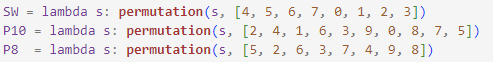
\includegraphics[width = 0.8\linewidth]{Imagens/Permutacoes.png}  
    \label{fig:Permutacoes}
\end{figure}

\begin{lstlisting}[language=Python]
def permutation(s: str, indices: list[int]) -> str:
    return ''.join(s[i] for i in indices)
\end{lstlisting}

\begin{figure}[h]
    \centering
    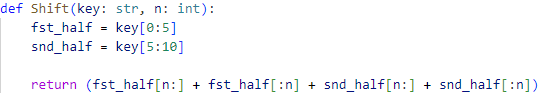
\includegraphics[width = 0.8\linewidth]{Imagens/Shift.png}  
    \label{fig:Shift}
\end{figure}

\begin{lstlisting}[language=Python]
def key_gen(key: str):
    intermediate_key = Shift((P10(key)), 1)

    K1 = P8(intermediate_key)
    K2 = P8(Shift(intermediate_key, 2))

    return (K1, K2)
\end{lstlisting}

Com a execução de todas essas operações, será obtido os seguintes valores a partir da chave recebida:
\begin{itemize}
  \item Intermediaria: 0000111000
  \item K1: 10100100
  \item K2: 01000011
\end{itemize}

\subsection{Permutação Inicial}
Para realizar a permutação inicial, é utilizada a mesma função de permutação utilizada na geração das sub-chaves definindo o array [1, 5, 2, 0, 3, 7, 4, 6]. Ao aplicar ao bloco de entrada a permutação inicial será obtido 11011101.

\subsection{Rodadas de Feistel}
Para realização das rodadas de Feistel, a entrada de 8 bits recebida é dividida ao meio (L e R) e é aplicada a equação $$f_{K}(L, R) = (L \  \oplus  \  F(R, \ SK), R)$$ e inverte o valor resultante, trocando L e R de lugar, usando a permutação [4, 5, 6, 7, 0, 1, 2, 3]. No modelo do SDES, serão realizadas apenas duas rodadas desse processo e por isso SK será, respectivamente, k1 e k2.

Das operações que serão utilizadas, falta apenas a definição da função F. Essa função tem como objetivo aplicar a \textbf{permutação de expansão}(EP) utilizando o array [3, 0, 1, 2, 1, 2, 3, 0], realizar o \textbf{XOR} entre a chave e a saída da permutação EP e por fim realizar a permutação P4 utilizando o array [1, 3, 2, 0] com os valores obtidos a partir das S-Boxes.

\begin{lstlisting}[language=Python, caption={Função F}]
def F(R: str, SK: str):
  s = XOR(EP(R), SK)
  return P4(S0[s[0] + s[3]][s[1] + s[2]] + S1[s[4] + s[7]][s[5] + s[6]])
\end{lstlisting}

A \blue{EP} é utilizada para transformar a entrada de 4 bits em uma saída de 8 bits, permitindo a realização do XOR com a chave. Já as \blue{S-Boxes} estabelecidas pelo algoritmo, que estão presentes na imagem \ref{fig:S-Boxes} e possuem valores para todas as combinações de 4 bits, permitem a conversão da entrada de 8 bits para uma saída	de 4 bits que será utilizada pela permutação P4.

\begin{figure}[h]
    \caption{S-Boxes}
    \centering
    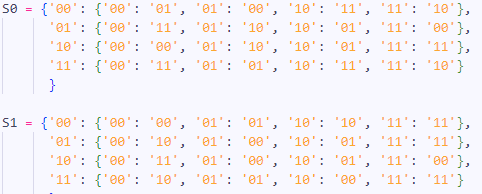
\includegraphics[width = 0.8\linewidth]{Imagens/S-Boxes.png}  
    \label{fig:S-Boxes}
\end{figure}

A fim de permitir um meio de comparar os resultados obtidos ao longo da $f_{k}$, o print do resultado das 2 rodadas de $f_{k}$ está presente na imagem \ref{fig:Feistel}.
\begin{figure}[h]
    \caption{Resultados intermediários das rodadas de Feistel}
    \centering
    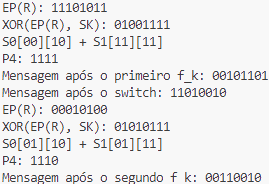
\includegraphics[width = 0.4\linewidth]{Imagens/Feistel.png}  
    \label{fig:Feistel}
\end{figure}

\newpage
\subsection{Permutação Final}

Para finalizar o algoritmo, é realizada uma permutação final a qual é a inversa da permutação inicialmente. Desse modo, a permutação utilizada é a [3, 0, 2, 4, 6, 1, 7, 5] e o resultado obtido seguindo todo o algoritmo será 10101000, que também é a \textbf{mensagem encriptada} resultante do S-DES.

Como definimos agora todo o processo para encriptar a mensagem, devemos definir como será feito para decriptar o \blue{ciphertext}. Dada a forma como o S-DES funciona, o processo de decriptação sera feito apenas invertendo a ordem de utilização das chaves, isto é, ao invés de k1 e k2 serão utilizadas k2 e k1 em $f_{k}$ obtendo o \blue{plaintext}. 
\newpage

\section{Modos de operação}
Ao iniciar o algoritmo, poderão ser utilizados dois modos de operação. Esses algoritmos são:

\subsection{ECB}
A técnica utilizada por esse modo de operação é bem simples, principalmente pela entrada fornecida será dividida em entradas do mesmo tamanho da utilizada pelo S-DES, ou seja, a entrada do ECB será de um conjunto de blocos de 8 bits que serão passados um a um para o algoritmo de encriptação do S-DES. Para isso, foi utilizada a função da imagem \ref{fig:ECB_Encript}.

\begin{figure}[h]
    \caption{ECB Encript}  
    \centering
    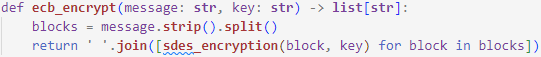
\includegraphics[width = 0.8\linewidth]{Imagens/ECB_Encrypt.png}  
    \label{fig:ECB_Encript}
\end{figure}

Para exemplificar, a mensagem fornecida ao programa ao passar pela função será convertida no array [11010111, 01101100, 10111010, 11110000]. Vale lembrar que esse \textbf{não} é o valor retornado pela função, pois este só será possível ao concatenar o resultado de cada bloco retornado ao utilizar o S-DES, que será 10101000 00001101 00101110 01101101.


\subsection{CBC}
Nesse modo de operação, além da mensagem dividida em blocos de 8 bits e da chave de 10 bits também será recebida um valor inicial (IV), que será utilizado para realizar a XOR com a mensagem a ser encriptada. Para isso foi utilizada a função:

\begin{lstlisting}[language=Python]
def XOR(s1:str, s2:str):
  return ''.join('1' if c1 != c2 else '0' for c1, c2 in zip(s1, s2))
\end{lstlisting}

Após a primeira iteração o valor utilizado para realizar o XOR com o bloco de mensagem será o valor retornado pela criptografia do SDES. Esse processo será repetido para todos os blocos de 8 bits da mensagem seguindo o loop da figura \ref{fig:CBC}. Os resultados obtidos em cada parte do CBC foram os apresentados na figura \ref{fig:CBC_Results}.

\begin{figure}[h]
    \caption{Algoritmo CBC}
    \centering
    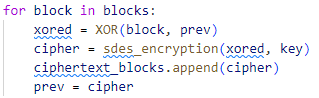
\includegraphics[width = 0.6\linewidth]{Imagens/CBC.png}  
    \label{fig:CBC}
\end{figure}

\begin{figure}[h]
    \caption{Resultados obtidos pelo CBC}
    \centering
    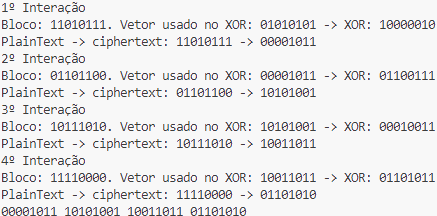
\includegraphics[width = 0.6\linewidth]{Imagens/CBC_Result.png}  
    \label{fig:CBC_Results}
\end{figure}

\section{Código}
O código está disponível no github pelo link: \href{https://github.com/Diehlgit/S-DES}{https://github.com/Diehlgit/S-DES}

\end{document}